\def\xxactivite{\ifprof Corrigé \else \ifcolle Colle \else TD \fi\fi}
\def\xxauteur{\textsl{Xavier Pessoles}}
\def\xxtitreexo{Micromanipulateur compact pour la chirurgie endoscopique ($\text{MC}^2\text{E}$)}
\def\xxsourceexo{\hspace{.2cm} \footnotesize{Concours Commun Mines Ponts 2016}}

\def\xxcompetences{%
\textsl{%
\textbf{Savoirs et compétences :}\\} \vspace{-.5cm}
\begin{itemize}
\item \textit{Res2.C18} : principe fondamental de la statique;
\item \textit{Res2.C19} : équilibre d’un solide, d’un ensemble de solides;
\item \textit{Res2.C20} : théorème des actions réciproques.
\end{itemize}
}

\def\xxauteur{\textsl{Xavier Pessoles}}

\def\xxfigures{
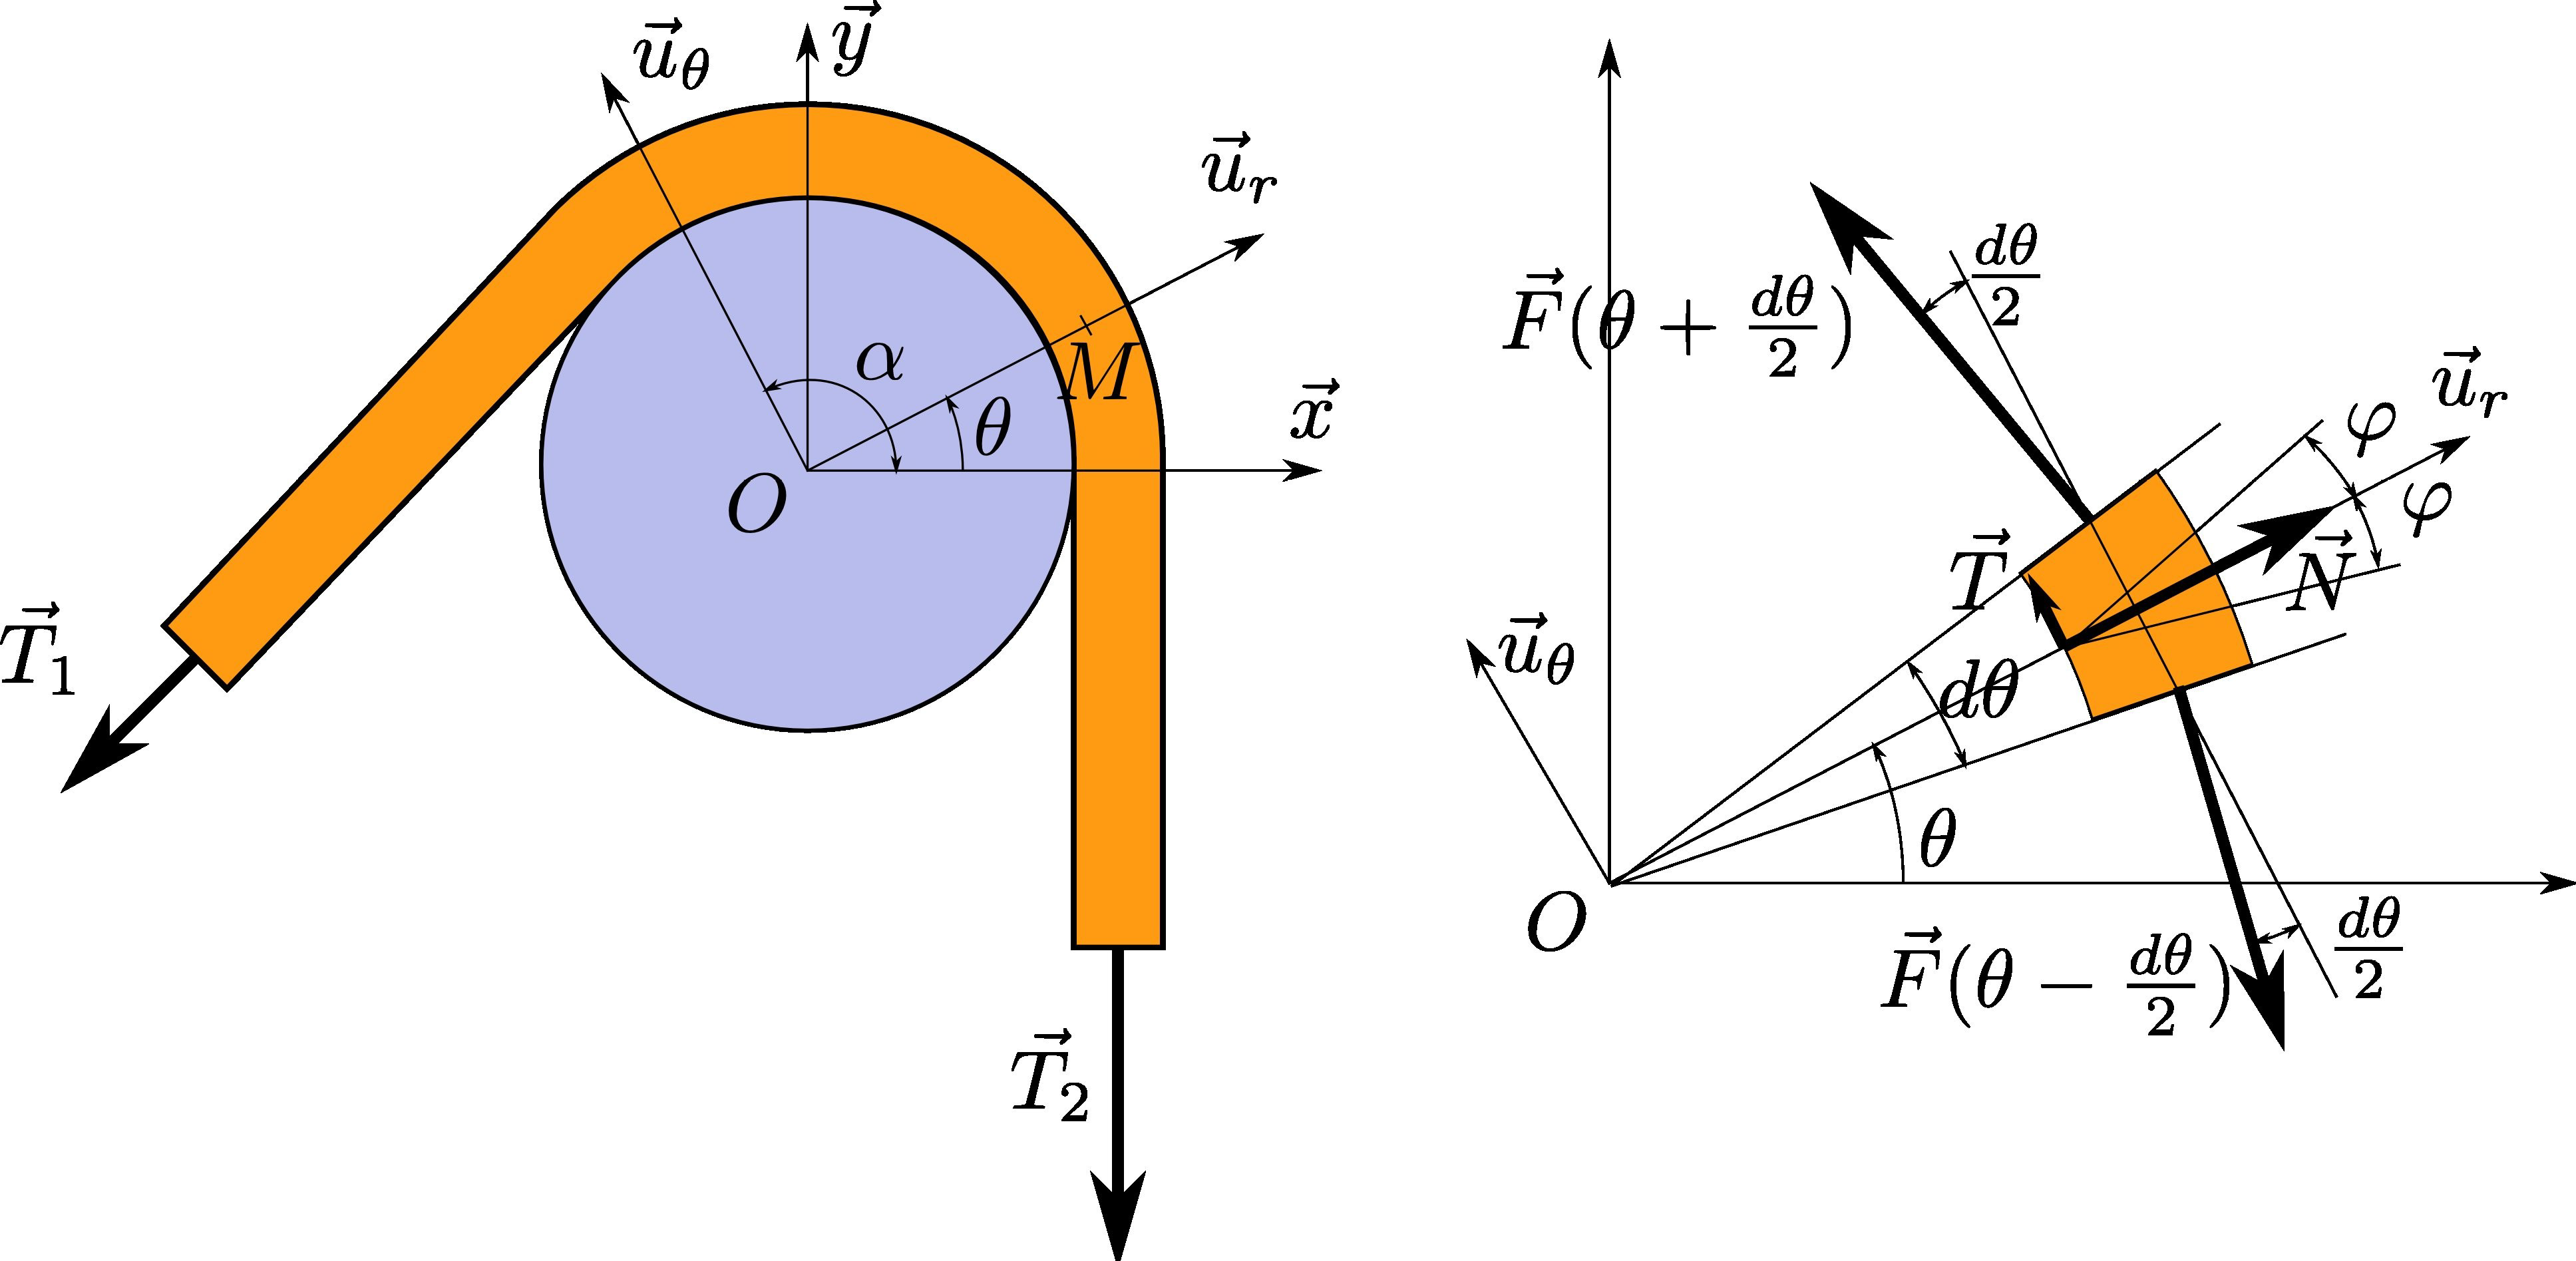
\includegraphics[width=.55\textwidth]{fig_01}
}%figues de la page de garde